\documentclass{beamer}

\mode<presentation>
{
	\usetheme{default}
	\usecolortheme{default} 
	\usefonttheme{default}  
	\setbeamertemplate{navigation symbols}{}
	\setbeamertemplate{caption}[numbered]
	\setbeamertemplate{footline}[frame number]
} 

\usepackage{url}
\usepackage{float}
\usepackage{caption}
\usepackage{graphicx}
\usepackage[utf8]{inputenc}
\usepackage{amsfonts}
\usepackage{times}
\usepackage[czech]{babel}

\author{Martin Bažík \\ xbazik00@stud.fit.vutbr.cz}
\title{Typografie a publikování \\ 5. projekt: Písmo}

\begin{document}
	\begin{frame}
		\titlepage
	\end{frame}
	
	\newpage
	
	
	\section{Písmo}
	
	\begin{frame}{Písmo}
		\transwipe
		\begin{itemize}
			\item Prvé písmo vzniklo už okolo roku 3200 pred naším letopočtom v \textbf{Mesopotámii}. 
			\item V rovnakom čase sa vyvinulo písmo v \textbf{Egypte}.
			\item Medzi písmom v Egypte a Mesopotámii sa objavujú podobnosti. 
			\item Medzi staré písma patrí taktiež čínske.
		\end{itemize}
		
		\vskip 1cm
		
%		\begin{block}{Examples}
%			Some examples of commonly used commands and features are included, to help you get started.
%		\end{block}
		
	\end{frame}
	
	
	
	\section{Príklad}
	
	\begin{frame}{Príklad}
		\transwipe
		\begin{figure}[H]
			\centering
			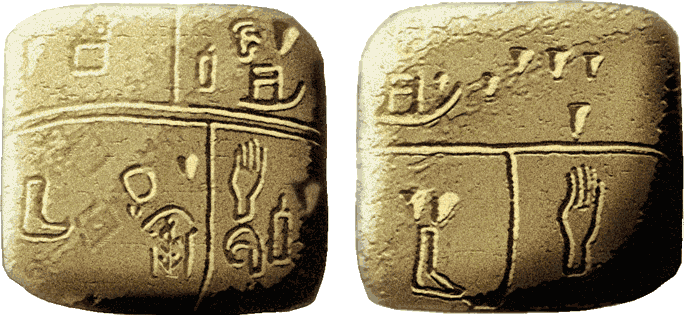
\includegraphics[scale=0.4]{Tab.png}	
			\caption{Klinové písmo zo Sumeru}
			\label{picKlin}
		\end{figure}
	\end{frame}
	
	
	\section{Základné delenie písma}
	
	\begin{frame}{Základné delenie písma}
		\transwipe
		\begin{itemize}
			\item Základné delenie:
			\begin{list}{$\circ$}{}
					\item Logografické
					\item Slabičné
					\item Abugida
					\item Spoluhláskové
					\item Pravé hláskové
			\end{list}
			\item Semaziografické delenie:
			\begin{list}{$\circ$}{}
				\item Predmetné písmo
				\item Piktografické písmo
				\item Ideografické písmo
			\end{list}		
		\end{itemize}
			
	\end{frame}


	\section{Prvé písma v Európe}
	
	\begin{frame}{Prvé písma v Európe}
		\transwipe
		\begin{itemize}
			\item Najstaršie písmo nájdené v \textbf{Európe} je datované pred \textbf{3500} rokmi.
			\item Toto písmo bolo nájdené v \textbf{Grécku} na hlinenej doske.
			\item Obsahuje viaceré znaky starého gréckeho \textbf{Lineárneho písma B}.
			\item Ďalšie európske písmo vzniklo taktiež v Grécku, nazýva sa \textbf{Alfabeta}.
			\item Vďaka alfabete pretrvali staré grécke báje a drámy až dodnes.
			\item Avšak väčšina európskych písem je založená na \textbf{Latinskom písme}.		
		\end{itemize}
			
	\end{frame}
		
	\section{Iklaina doska}
	
	\begin{frame}{Iklaina doska}
		\transwipe
		\begin{figure}[H]
			\centering
			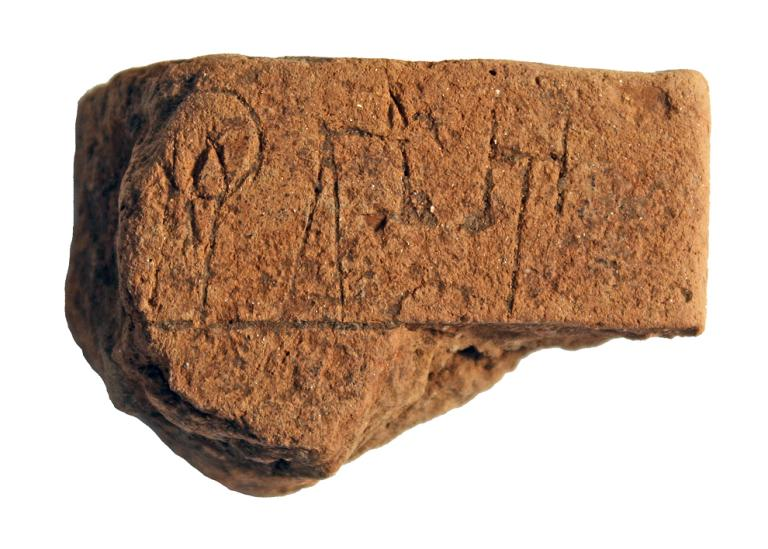
\includegraphics[scale=0.3]{tabletin}	
			\caption{Iklaina doska, najstaršie písmo v Európe}
			\label{picKlin}
		\end{figure}
	\end{frame}
		


	\section{Zdroje}
	\transwipe
	\begin{frame}{Zdroje}
		\transwipe
		\begin{itemize}
			\scriptsize{
				\item \url{https://en.wikipedia.org/wiki/History_of_writing}
				\item \url{https://sk.wikipedia.org/wiki/P\%C3\%ADsmo_(jazykoveda)}
				\item \url{http://phys.org/news/2011-04-oldest-evidence-europe.html}
				\item \url{http://news.nationalgeographic.com/news/2011/03/110330-oldest-writing-europe-tablet-greece-science-mycenae-greek/}
			}
		\end{itemize}
	\end{frame}


\end{document}
